\documentclass[11pt]{article}

\usepackage{float}
\usepackage{hyperref}
\usepackage{graphicx}
% formatting
\usepackage{verbatim}
\usepackage{moreverb}
\usepackage{minted}
\usepackage{parskip}
\usepackage{amsmath}
\usepackage[listings]{tcolorbox}
\usepackage{enumerate}
\usepackage{tikz}
\usetikzlibrary{arrows,automata, positioning}
\let\verbatiminput=\verbatimtabinput
\def\verbatimtabsize{4\relax}

\newcommand{\RepoRootPath}{fpga\_labs\_fa19}

\tcbset{
texexp/.style={colframe=black, colback=lightgray!15,
         coltitle=white,
         fonttitle=\small\sffamily\bfseries, fontupper=\small, fontlower=\small},
     example/.style 2 args={texexp,
title={Question \thetcbcounter: #1},label={#2}},
}

\newtcolorbox{texexp}[1]{texexp}
\newtcolorbox[auto counter]{texexptitled}[3][]{%
example={#2}{#3},#1}

\setlength{\topmargin}{-0.5in}
\setlength{\textheight}{9in}
\setlength{\oddsidemargin}{0in}
\setlength{\evensidemargin}{0in}
\setlength{\textwidth}{6.5in}

% Useful macros

\newcommand{\note}[1]{{\bf [ NOTE: #1 ]}}
\newcommand{\fixme}[1]{{\bf [ FIXME: #1 ]}}
\newcommand{\wunits}[2]{\mbox{#1\,#2}}
\newcommand{\um}{\mbox{$\mu$m}}
\newcommand{\xum}[1]{\wunits{#1}{\um}}
\newcommand{\by}[2]{\mbox{#1$\times$#2}}
\newcommand{\byby}[3]{\mbox{#1$\times$#2$\times$#3}}


\newenvironment{tightlist}
{\begin{itemize}
 \setlength{\parsep}{0pt}
 \setlength{\itemsep}{-2pt}}
{\end{itemize}}

\newenvironment{titledtightlist}[1]
{\noindent
 ~~\textbf{#1}
 \begin{itemize}
 \setlength{\parsep}{0pt}
 \setlength{\itemsep}{-2pt}}
{\end{itemize}}

% Change spacing before and after section headers

\makeatletter
\renewcommand{\section}
{\@startsection {section}{1}{0pt}
 {-2ex}
 {1ex}
 {\bfseries\Large}}
\makeatother

\makeatletter
\renewcommand{\subsection}
{\@startsection {subsection}{1}{0pt}
 {-1ex}
 {0.5ex}
 {\bfseries\normalsize}}
\makeatother

% Reduce likelihood of a single line at the top/bottom of page
\clubpenalty=2000
\widowpenalty=2000

% Other commands and parameters
\pagestyle{myheadings}
\setlength{\parindent}{0in}
\setlength{\parskip}{10pt}

% Commands for register format figures.
\newcommand{\instbit}[1]{\mbox{\scriptsize #1}}
\newcommand{\instbitrange}[2]{\instbit{#1} \hfill \instbit{#2}}

% Break lines on texttt text on underscores
% See: https://tex.stackexchange.com/questions/315369/how-to-deal-with-bad-line-wrapping-of-texttt
\newcommand*\ttvar[1]{\texttt{\expandafter\dottvar\detokenize{#1}\relax}}
\newcommand*\dottvar[1]{\ifx\relax#1\else
  \expandafter\ifx\string_#1\string_\allowbreak\else#1\fi
  \expandafter\dottvar\fi}

\graphicspath{{./figs/}}
\newcommand{\itwos}{I\textsuperscript{2}S}

\begin{document}

\def\PYZsq{\textquotesingle}
\title{\vspace{-0.4in}\Large \bf EECS 151/251A FPGA Lab 6:\\FIFOs, UART Piano\vspace{-0.1in}}

\author{Prof. Borivoje Nikolic and Prof. Sophia Shao \\
TAs: Cem Yalcin, Rebekah Zhao, Ryan Kaveh, Vighnesh Iyer \\ Department of Electrical Engineering and Computer Sciences\\
College of Engineering, University of California, Berkeley}
\date{}
\maketitle

\newcommand{\headertext}{EECS 151/251A FPGA Lab 6: FIFOs, UART Piano}
\markboth{\headertext}{\headertext}
\thispagestyle{empty}

\section{Introduction}
Run \verb|git pull| in \texttt{\RepoRootPath}.
Copy the modules you created in the previous lab to this lab:
\begin{minted}{text}
  cd fpga_labs_fa19
  cp lab5/src/synchronizer.v lab6/src/.
  cp lab5/src/debouncer.v lab6/src/.
  cp lab5/src/edge_detector.v lab6/src/.
  cp lab5/src/tone_generator.v lab6/src/.
  cp lab5/src/music_streamer.v lab6/src/.
  cp lab5/src/uart_transmitter.v lab6/src/.
\end{minted}

\subsection{Overview}
In this lab, you will integrate the UART created in Lab 5 and the tone generator from the previous labs to create a ``piano''.
In the first part, you will build a synchronous FIFO and verify its functionality using a block-level testbench.
Then you will use a FIFO to bridge the UART with an FSM that plays notes with a fixed duration send from your computer.
You will extend the FSM to support playing variable length notes.
In the final part, you will extend the tone generator's volume control capability and implement a note amplitude envelope to resemble a real instrument.

Here is an overview of the entire system in \verb|z1top| we are going to build.
You may find it useful to refer to this block diagram while doing this lab.

\begin{figure}[H]
    \centerline{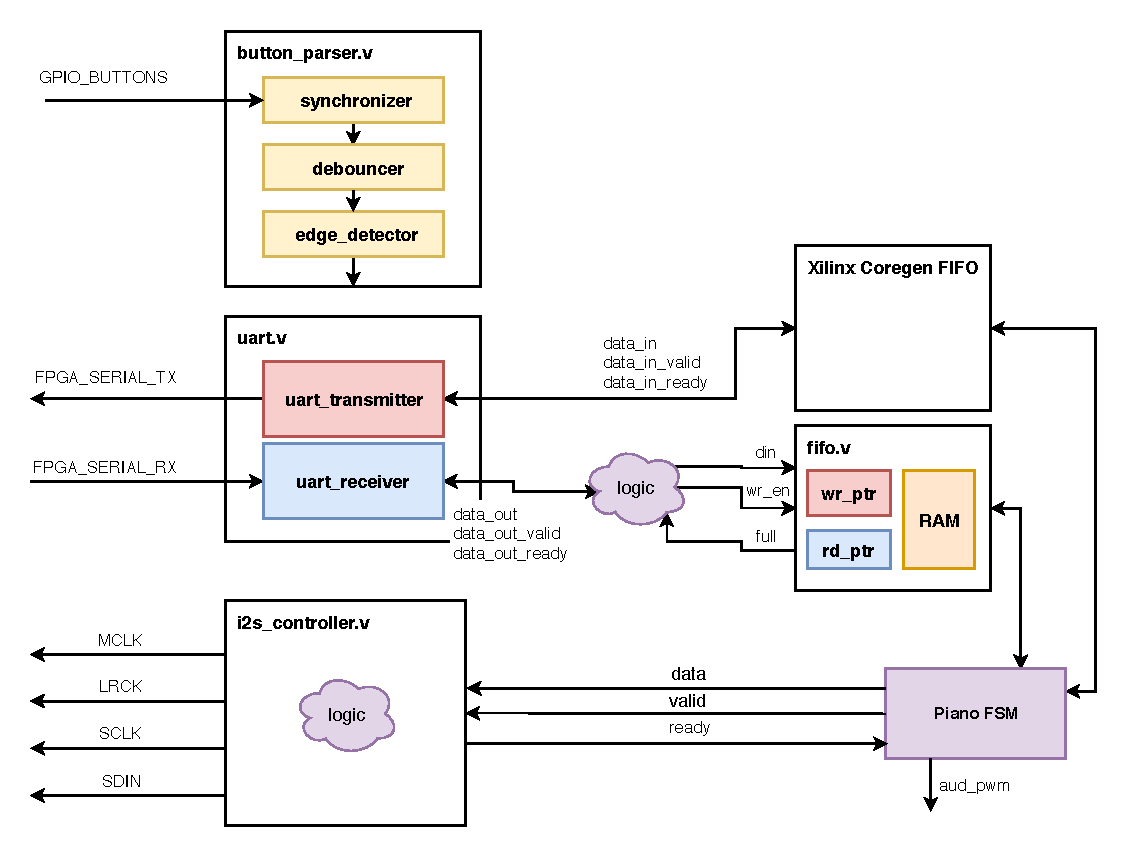
\includegraphics[width=\textwidth]{Lab6_Block_Diagram.pdf}}
\end{figure}

\section{Buliding a Synchronous FIFO}
A FIFO (first in, first out) data buffer is a circuit that allows data elements to be queued through a write interface, and read out sequentially by a read interface.
The FIFO we will build in this section will have both the read and write interfaces clocked by the same clock; this circuit is known as a synchronous FIFO.

\subsection{FIFO Functionality}
A FIFO is implemented with a circular buffer (2D reg) and two pointers: a read pointer and a write pointer.
These pointers address the buffer inside the FIFO, and they indicate where the next read or write operation should be performed.
When the FIFO is reset, these pointers are set to the same value.

When a write to the FIFO is performed, the write pointer increments and the data provided to the FIFO is written to the buffer.
When a read from the FIFO is performed, the read pointer increments, and the data present at the read pointer's location is sent out of the FIFO.

A comparison between the values of the read and write pointers indicate whether the FIFO is full or empty.
You can choose to implement this logic as you please.
The \verb|Electronics| section of the \href{https://en.wikipedia.org/wiki/FIFO_(computing_and_electronics)}{FIFO Wikipedia article} will likely aid you in creating your FIFO.

Here is a block diagram of the FIFO you should create from page 103 of the \href{https://www.xilinx.com/support/documentation/ip_documentation/fifo_generator_ug175.pdf}{Xilinx FIFO IP Manual}.

\begin{center}
    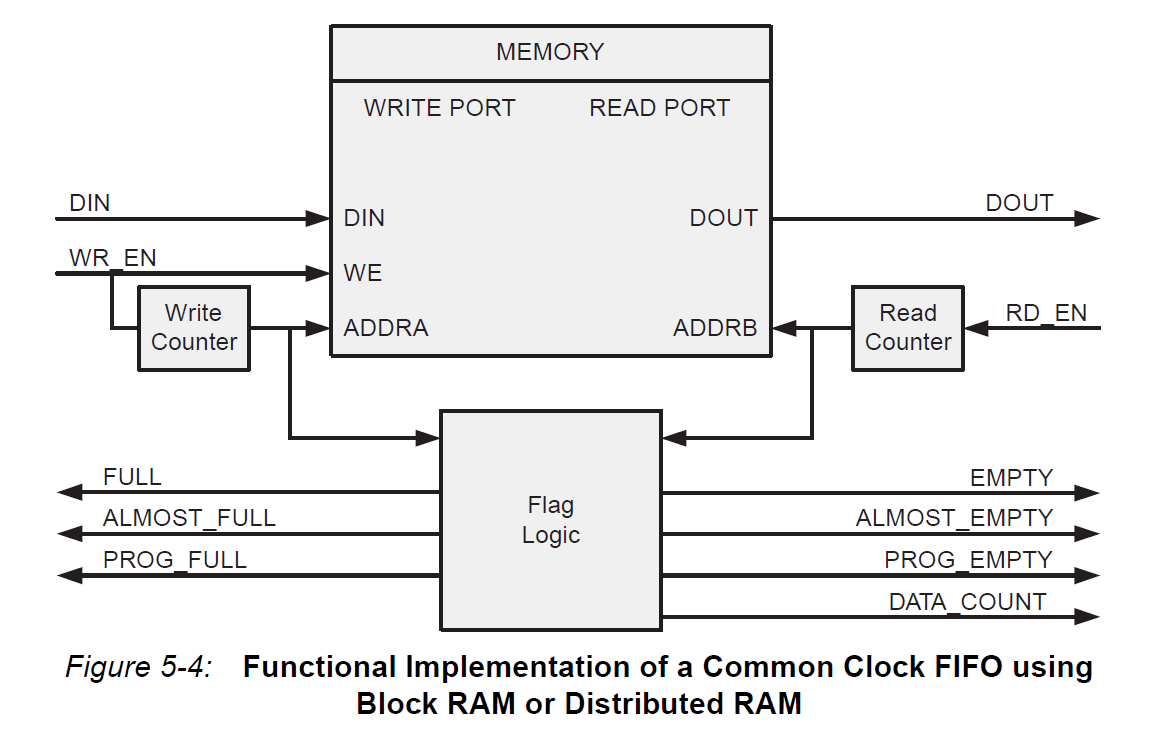
\includegraphics[height=7cm]{sync_fifo_diagram.png}
\end{center}

The interface of our FIFO will contain a subset of the signals enumerated in the diagram above.

\subsection{FIFO Interface}
Look at the FIFO skeleton in \verb|src/fifo.v|.

The FIFO is parameterized by:
\begin{itemize}
    \item \verb|data_width| - The number of bits per entry in the FIFO
    \item \verb|fifo_depth| - The number of entries in the FIFO.
    \item \verb|addr_width| - Calculated as the width of the read and write pointers.
\end{itemize}

The common FIFO signals are:
\begin{itemize}
    \item \verb|clk| - Clock used for both read and write interfaces of the FIFO.
    \item \verb|rst| - Reset (synchronous with \verb|clk|); should force the FIFO to become empty.
\end{itemize}

The FIFO write interface consists of:
\begin{itemize}
    \item \verb|input wr_en| - When this signal is high, on the rising edge of the clock, the data on \verb|din| should be written to the FIFO.
    \item \verb|input [data_width-1:0] din| - The data to be written to the FIFO.
    \item \verb|output full| - When this signal is high, the FIFO is full.
\end{itemize}

The FIFO read interface consists of:
\begin{itemize}
    \item \verb|input rd_en| - When this signal is high, on the rising edge of the clock, the FIFO should output the data indexed by the read pointer on \verb|dout|
    \item \verb|output [data_width-1:0] dout| - The data that was read from the FIFO after the rising edge on which \verb|rd_en| was asserted
    \item \verb|output empty| - When this signal is high, the FIFO is empty.
\end{itemize}

\subsection{FIFO Timing}
The FIFO that you design should conform to the specs above.
To further, clarify here are the read and write timing diagrams from the \href{https://www.xilinx.com/support/documentation/ip_documentation/fifo_generator_ug175.pdf}{Xilinx FIFO IP Manual}.
These diagrams can be found on pages 105 and 107.
Your FIFO should behave similarly.

\begin{figure}[H]
    \minipage{0.48\textwidth}
    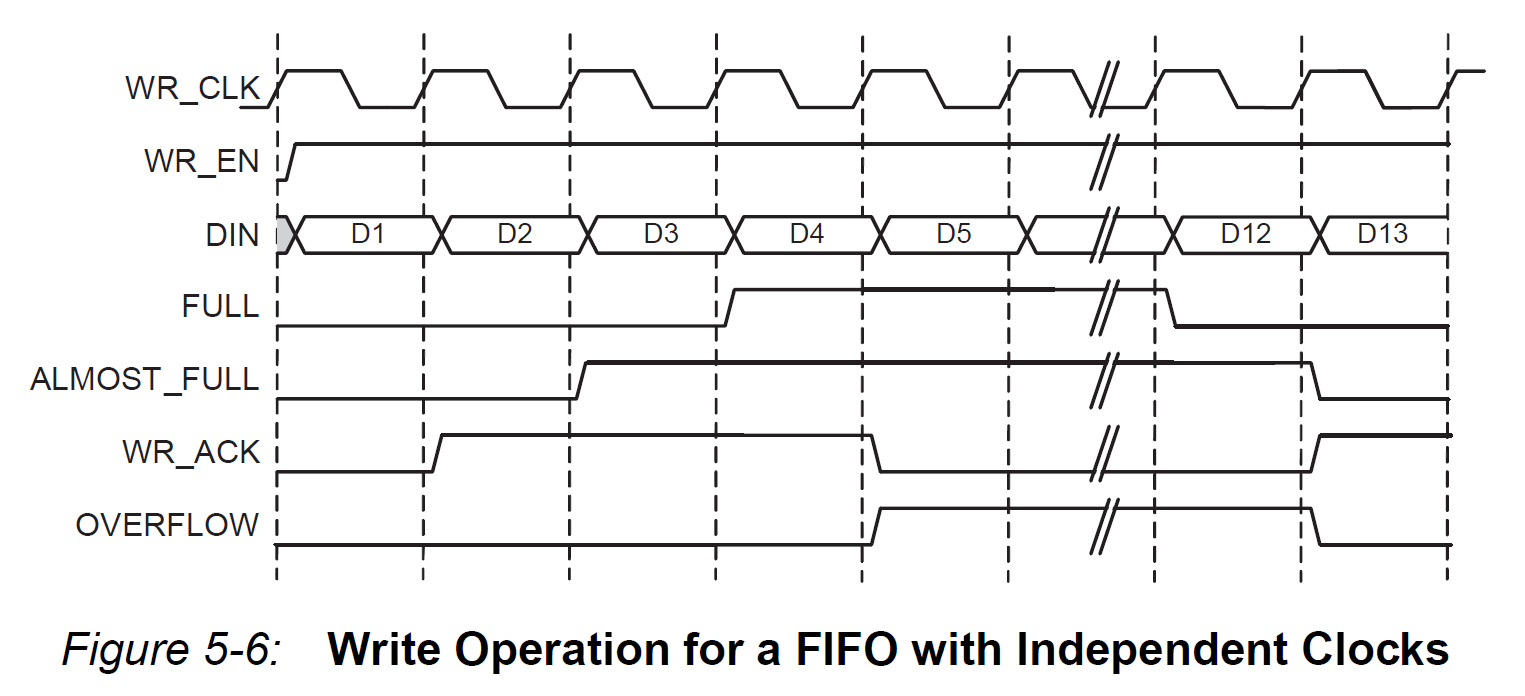
\includegraphics[width=\linewidth]{sync_fifo_write_operation.png}
    \endminipage\hfill
    \minipage{0.48\textwidth}
    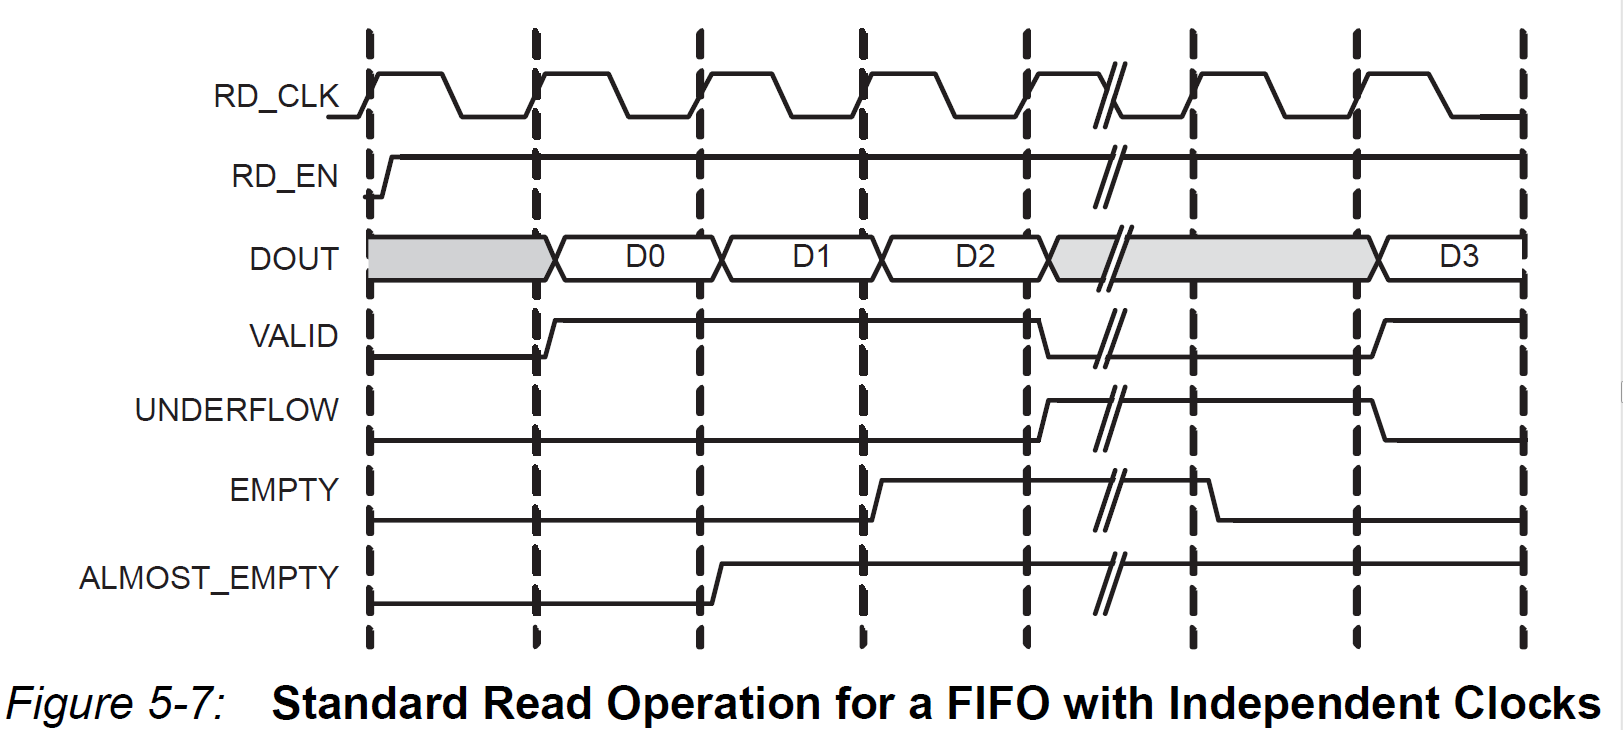
\includegraphics[width=\linewidth]{sync_fifo_read_operation.png}
    \endminipage
\end{figure}

Your FIFO doesn't need to support the \verb|ALMOST_FULL|, \verb|WR_ACK|, or \verb|OVERFLOW| signals on the write interface and it doesn't need to support the \verb|VALID|, \verb|UNDERFLOW|, or \verb|ALMOST_EMPTY| signals on the read interface.

\subsection{FIFO Testing}
We have provided a testbench in \verb|sim/fifo_testbench.v|.

The testbench performs the following test sequence:
\begin{enumerate}
    \item Checks initial conditions after reset (FIFO not full and is empty)
    \item Generates random data which will be used for testing
    \item Pushes the data into the FIFO, and checks at every step that the FIFO is no longer empty
    \item When the last piece of data has been pushed into the FIFO, it checks that the FIFO is not empty and is full
    \item Verifies that cycling the clock and trying to overflow the FIFO doesn't cause any corruption of data or corruption of the full and empty flags
    \item Reads the data from the FIFO, and checks at every step that the FIFO is no longer full
    \item When the last piece of data has been read from the FIFO, it checks that the FIFO is not full and is empty
    \item Verifies that cycling the clock and trying to underflow the FIFO doesn't cause any corruption of data or corruption of the full and empty flags
    \item Checks that the data read from the FIFO matches the data that was originally written to the FIFO
    \item Prints out test debug info
\end{enumerate}

This testbench tests one particular way of interfacing with the FIFO.
Of course, it is not comprehensive, and there are conditions and access patterns it does not test.
We recommend adding some more tests to this testbench (or writing a new testbench) to verify your FIFO performs as expected. Here are a few tests to try:

\begin{itemize}
    \item Several times in a row, write to, then read from the FIFO with no clock cycle delays.
      This will test the FIFO in a way that it's likely to be used when buffering user I/O.

    \item Try writing and reading from the FIFO on the same cycle.
      This will require you to use fork/join to run two threads in parallel.
      Make sure that no data gets corrupted.
\end{itemize}

\section{Building the Piano}
The piano interfaces the UART with the tone generator.
Its job is to fetch notes sent from the UART, convert them to a \verb|tone_switch_period|, and send them to the \verb|tone_generator| for a fixed note length.
This is the `piano' module in the diagram in the lab intro.

Fill in \verb|src/piano.v|.
It has access to the UART transmitter FIFO, the UART receiver FIFO, and the \verb|tone_generator| inputs.
It also has access to a reset signal and the other buttons.
The piano should implement the following functionality:

\begin{itemize}
    \item When the UART receiver FIFO contains a character, the FSM should pull the character from the FIFO and echo it back without modification through the UART transmitter FIFO.

    \item Once a character is pulled, its corresponding \verb|tone_switch_period| should be read from the supplied \verb|piano_scale_rom.v|.

    \item For a fixed amount of time (\verb|note_length|), the tone should be played by sending it to the \verb|tone_generator|.

    \item The \verb|note_length| should default to 1/5th of a second, and can be changed by a fixed amount with the buttons.
      Let \verb|buttons[0]| increase/decrease the \verb|note_length| depending on the value of \verb|switches[0]|.
      This is similar to the runtime tempo modification you implemented in the \verb|music_streamer|.

    \item Through doing all of this, your FSM should take care to ensure that if a FIFO is full, that it waits until it isn't full before pushing through data.

    \item You can use the \verb|leds| output for debugging
\end{itemize}

You don't need to design the \verb|piano| as an explicit FSM with states; the design is entirely up to you.

A ROM containing mappings from ASCII character codes to the \verb|tone_switch_period| of the note to be played can be found in \verb|src/piano_scale_rom.v|.
If you wish to re-generate this file, use these commands:

\begin{minted}{bash}
cd lab6
python scripts/piano_scale_generator.py scale.txt
python scripts/rom_generator.py scale.txt src/piano_scale_rom.v 256 24
# Modify piano_scale_rom.v to change the module name to 'piano_scale_rom'
\end{minted}

It is possible that the UART receiver FIFO can fill up with samples so fast that the piano can't keep up; similar overflow conditions are possible with other parts of this system.
You don't need to concern yourself with detecting 'backpressure' on the entire system and can just assume that your FIFOs are large enough to buffer all the user input.

\subsection{Modify z1top}
Open up \verb|z1top.v| and modify it to include the new modules you wrote.
Wire up the FIFOs and your piano + tone generator according to the block diagram in the lab intro.
You will have to add a few lines of logic (purple cloud) representing the bridge between the ready/valid interface and the FIFO's \verb|rd_en, wr_en, full, empty| interface.

Make sure that you parameterize your FIFOs properly so that they have the proper \verb|data_width|.
You can make your FIFOs as deep as you want, but 8 should be enough.

\section{Writing a System-Level Testbench}
This design involves quite a few moving parts that communicate with each other.
We want to make sure that the complete integration of our system works as expected.
To that end, you will have to write a system-level testbench that stimulates the top-level of your design and observes the top-level outputs to confirm correct behavior.

We have provided a template for a system testbench in \verb|sim/system_testbench.v|.
Fill in the \verb|initial| block to test all the parts of the piano.

To make the waveform shorter and easier to debug, it is suggested that you change the \verb|note_length| default value in the \verb|piano| to something much smaller than 1/5th of a second, just for testing.

\section{FPGA Testing}
Generate a bitstream and program the FPGA as usual.
Read the synthesis and implementation reports (\ttvar{build/synth/synth.log}) to see if there are any unexpected warnings.

You should watch out specifically for warnings like ``found x-bit latch'' or ``x signal unconnected'' or ``x signal assigned but never used''.
If you see that the synthesis tool inferred a latch, you should definitely fix that warning by completing any if-elseif-else or case statements that don't have a default signal assignment.
The other 2 warning types are dependent on your design and you should ignore them only if you know they are expected.

Once you put your design on the FPGA you can send data to the on-chip UART by using \verb|screen $SERIALTTY 115200|.
The piano keys are mapped such that `z' through `$<$' go from C3 to C4 (middle C) and `q` through 'i' go from C4 to C5.
Holding down shift moves the lower row's octave down and the upper row's octave up.

You can use the 1st button to change the \verb|note_length| of your piano.
You should test the case where you make the \verb|note_length| long, and fill up your UART FIFO by typing really fast.
Then watch your FIFO drain slowly as each note is played for \verb|note_length| time.

\textbf{For Checkoff:} Save the bitstream of the fixed note length piano by copying the \verb|build| directory, so it can be used during checkoff:
\begin{minted}{bash}
cp -r build build_fixed
\end{minted}

\section{Variable Note Lengths}
We would like to set the length of each note based on how long each key is pressed, instead of having a fixed note length.
We have provided a Python script that captures keyboard keyup/keydown events and translates them into 2 UART frames (a packet) indicating whether a note should begin playing or finish playing:

\begin{itemize}
  \item A key press causes 2 UART frames to be sent in order: \texttt{0x80, character} where \texttt{character} is the key that was pressed
  \item A key release causes 2 UART frames to be sent in order: \texttt{0x81, character} where \texttt{character} is the key that was released
\end{itemize}

Once you get a key press packet, you should begin playing the note associated with \texttt{character}, similar to before.
If you get a key release packet that has a matching \texttt{character} with the note being played, you should stop playing it.

If you're playing a note and you get key press packet, you should throw it away.
If you're playing a note and get a key release packet for a different \texttt{character}, you should throw it away.

You don't have to drive any characters into the UART TX in this part.
Drive an LED indicating when a note is being played.

\subsection{Testing}
Modify the \verb|system_testbench| to test variable length note playing, and test the edge cases where multiple keys are pressed before they are released.

Program it on the FPGA as usual.
Then run \verb|python3 scripts/piano.py| which captures keyboard events and sends them to the FPGA via UART.
You can play the same notes as beforehand.

\subsubsection{Testing Locally}
First, install some python packages (\verb|pip3 install pynput pyserial|).

If you're using Linux or OSX, you may have to launch the \verb|piano.py| script with \verb|sudo|.
On Ubuntu, you may have to run this line first if you \href{https://stackoverflow.com/questions/48833451/no-protocol-specified-when-running-a-sudo-su-app-on-ubuntu-linux}{get an X11 error} (\verb|xhost si:localuser:root|).

If you're on Windows, in addition to installing the Python packages, you should modify the \verb|scripts/piano.py| file (line 10) with the COM port assigned to the USB-UART device (according to the Device Manager).

%\section{Fine Volume Control + Amplitude Envelope}
% Too much work
% Implement a partial ADSR (attack, delay, sustain, release) envelope of your output waveforms. Here is a reference link \url{https://en.wikipedia.org/wiki/Synthesizer#Attack_Decay_Sustain_Release_.28ADSR.29_envelope}. You only need to implement an attack and release volume rolloff, and can use a single volume level for both the delay and sustain portions of your waveform. You should include some way of changing the attack and release periods (either through the rotary encoder or buttons).

\section{Checkoff Tasks}
\begin{enumerate}
  \item Show the system-level testbench you wrote and its methodology for testing your piano's functionality.
  \item Show the output waveform of your testbench and explain how data moves through your system.
  \item Demonstrate the variable note length piano working on the FPGA.
  \item For the fixed note length piano, prove the existence of your UART RX and TX FIFOs by making the note length long, then pressing multiple keys in quick succession, filling the RX FIFO and, then seeing the notes drain out slowly into the piano.

    You can program the FPGA using your saved bitstream with:
\begin{minted}{bash}
cp -r build build_variable
rm -rf build
mv build_fixed build
make program-force
\end{minted}
\end{enumerate}

\subsection{Lab Report}
No lab report!

\section*{Ackowlegement}
This lab is the result of the work of many EECS151/251 GSIs over the years including:
\begin{itemize}
\item Sp12: James Parker, Daiwei Li, Shaoyi Cheng
\item Sp13: Shaoyi Cheng, Vincent Lee
\item Fa14: Simon Scott, Ian Juch
\item Fa15: James Martin
\item Fa16: Vighnesh Iyer
\item Fa17: George Alexandrov, Vighnesh Iyer, Nathan Narevsky
\item Sp18: Arya Reais-Parsi, Taehwan Kim
\item Fa18: Ali Moin, George Alexandrov, Andy Zhou
\end{itemize}

\end{document}
